%\title{Article HW Template}

\documentclass[12pt]{article}
\usepackage[paper=a4paper,top=1in, bottom=1in, right=1in, left=.7in]{geometry}
\usepackage{amsthm, amssymb, amsfonts, amsmath}
\usepackage{graphicx}
\usepackage{tikz}
\usetikzlibrary{calc,shapes}
\usepackage{enumitem}
\usepackage{mathtools}
\usepackage{mathrsfs}
\usepackage{tikz-cd}
\usepackage{hyperref, mathabx}
\usepackage{algorithm}
\usepackage{algpseudocode}
\renewcommand{\algorithmicrequire}{\textbf{Input:}}
\renewcommand{\algorithmicensure}{\textbf{Output:}}

\newcommand{\boxitem}[2]{\vspace{.55cm}
	\item[#1]
	\leavevmode
	\strut
	\vadjust{%%
		\noindent
		\raisebox{\dimexpr\dp\strutbox+\ht\strutbox+1ex}[0pt][0pt]{\tikzmark{bl}}}%%
	#2
	
	\leavevmode
	\vadjust{%
		\noindent
		\hspace*{\dimexpr\textwidth+1ex}\tikzmark{br}}%%
	
	\tikz[overlay,remember picture]{\draw[black]
		(bl) rectangle
		(br);}}

\newcommand{\tikzmark}[1]{\tikz[overlay,remember picture] \node (#1) {};}

\newcommand{\R}{\mathbb{R}}
\newcommand{\Q}{\mathbb{Q}}
\newcommand{\Z}{\mathbb{Z}}
\newcommand{\N}{\mathbb{N}}
\newcommand{\p}{\mathbb{P}}
\newcommand{\E}{\mathbb{E}}
\newtheorem*{lemma}{Lemma}
\newtheorem{llemma}{Lemma}
\newtheorem*{theorem}{Theorem}
\newtheorem*{prop}{Proposition}

\begin{document}
	\null\hfill\begin{tabular}[t]{r@{}}
		Nikolas Mavrogeneiadis - 161014\\
		gravitorious \\
		University Of West Attica \\
		Department of Informatics and Computer Engineering\\
		Professor: Panagiotis Rouvelas\\
		\today
	\end{tabular}
	\\
	\centerline{\scshape{Graph Theory-Exercise Set 1}}
	
	\begin{enumerate}[listparindent=1.5em,
		parsep = 0pt]
		
	\boxitem{1.}{
		Prove that at least two vertices have the same degree in any simple graph with $n(vertices)>2$.
	}
		\underline{Proof:}
		Let $G(V,E)$ be a simple graph that for every pair of vertices $v_1$ and $v_2$ we have that $d(v1) \neq d(v2)$ where $d(v)$ is the degree of vertex $v$. Then, each vertex has a degree from the set $\{0, 1, 2, ..., n-1\}$. This means that there is a vertex with degree 0 and vertex with degree n - 1. But this is a contradiction.
		
	\boxitem{2.}{
		Let H be subgraph of G. Which of the following statements is correct? \\
		$i) d(G) \geq d(H)$ \\
		$ii) D(G) \geq D(H)$ \\
	}
		\underline{Proof:}
		For the $i)$ it is easy to find a counterexample. Let G with $d(G) = 1$ and there are only one vertex $v_1$ with this degree. We can delete this vertex and the new subgraph H will have $d(H) = 2$. \\
		\begin{figure}[h]
			\centering
			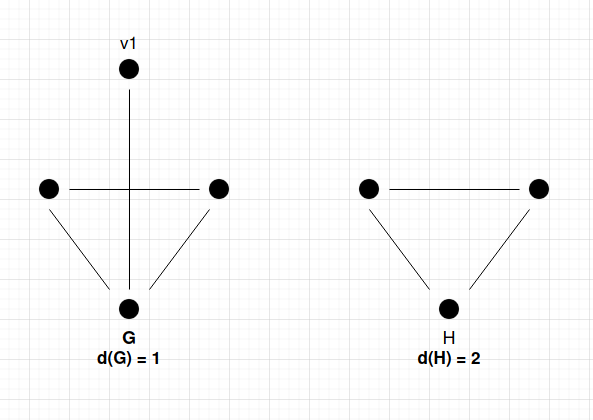
\includegraphics[width=0.55\textwidth]{pic1}
			\caption{A counterexample}
			\label{fig:mesh1}
		\end{figure}\\
		For the $ii)$ assume that exists $G(V,E)$ and its subgraph $H(\hat{V}, \hat{E})$ with $D(G) < D(H)$. This means that H contains an edge that G not. But this is a contradiction because $\hat{E} \subseteq E$.
		
	\boxitem{3.}{
		Prove that doesn't exist a 2k-regular graph with bridge.
	}
	\underline{Proof:} Assume that exists a 2k-regular graph with bridge. This means that each vertex has an even degree. If we delete the bridge edge, then we will have two components. Each of these has exactly one vertex with odd degree and with the rest having even degree. This means that the sum of degrees of all vertices for each component is odd number. This is a contradiction because we know that the sum of degrees is an even number.
	
	\boxitem{4.}{
		Prove that for every finite graph G, exists $m>0$ with $G^{m+1} = G^{m}$.
	}
	\underline{Proof:} Let diameter(d) be the maximum distance of G between any pair of vertices. Let the pair of vertices $(v_{1}, v_{2})$ be that with the maximum distance. Then it is easy to see that $G^{d}$ is a complete graph because if it isn't, the path from $v_{1}$ to $v_{2}$ is more than one, so d wasn't the maximum distance. A contradiction. Let $m:=d$. Then $G^{m+1}$ is the same complete graph. So $G^{m} = G^{m+1}$.
	
	\boxitem{5.}{
		Prove that for every simple graph G(V,E) with $n = |V|$ and $d(G)\geq\frac{n-1}{2}$ is connected.
	}
	\underline{Proof:} Suppose that G is not connected. Then G has at least two components. Each of these have at least one vertex with degree $\frac{n-1}{2}$. Now counting all the vertices of graph (including the two vertices) we see that $|V| = \frac{n-1}{2} + \frac{n-1}{2} + 1 + 1 = n+1$. A contradiction. 
	
	\newpage
	
	\boxitem{6.}{
		Give an efficient algorithm that takes as input a degree sequence and construct a simple graph from that sequence.  Run the algorithm with input $(5,4,3,3,2,2,1)$.
	}
	\underline{Proof:} For the algorithm we have used the fact that obtained from Havel-Hakimi theorem, that from a degree sequence, a $v_{i}$ vertex connects with the next $d_{i}$ vertices.\\
	\begin{algorithm}
		\caption{Construct graph from a degree sequence}
		\label{alg:cap}
		
		\begin{algorithmic}
			\Require A degree sequence $s = (d_{1}, d_{2},...,d_{k})$ with $d_{1} \geq d_{2} ... \geq d_{k}, k \geq 1$
			\Ensure A graph $G(V,E)$ from sequence s
			\State $vertices[ ] := $ List that contains the vertices  $v_{i}$ for each $s_{i}=d_{i}, 1 \leq i \leq k$
			\State $e[] := empty$ \Comment{Contains pairs with edges}
			\While{all elements from $s$ is non-zero}
				\If{$s$ contains negative number}
					\State print "Invalid degree sequence"
					\State exit
				\EndIf
			
				\State $i:=1$
				\For{\texttt{$j:=1$ to $d_{i}$}}
					\State e.push(create\_edge($vertices[i], vertices[i+j]$))
					\State $s[i+j] = s[i+j] - 1$
				\EndFor
				\State $s[i] = 0$
				\State $i:= i + 1$
				\State sort(s, vertices, i) \Comment{Sort s with decreasing order from i to k and simultaneously the vertices list with the same order}
			\EndWhile
		\end{algorithmic}
	\end{algorithm} 

	The following figure shows what lists $s$ and $vertices$ contain on each loop for the input $(5,4,3,3,2,2,1)$.\\
	\begin{figure}[h]
		\centering
		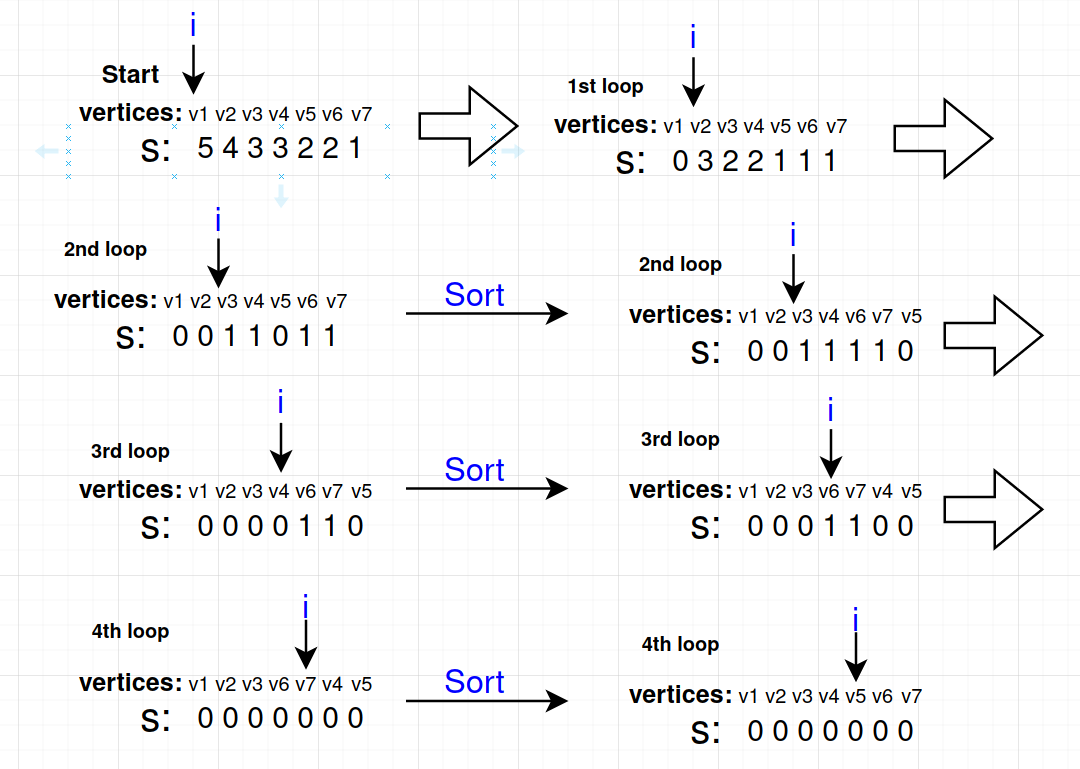
\includegraphics[width=0.85\textwidth]{pic2}
		\caption{vertices and s for input (5,4,3,3,2,2,1)}
		\label{fig:mesh1}
	\end{figure}\\
	 
	\newpage
	\boxitem{7.}{
		Prove that for every graph $G$, this graph or its complement $\tilde{G}$ is connected.
	}
	\underline{Proof:} Suppose that G is disconnected. Let two vertices $u,v \in V(G)$. Then these vertices will belong to the same component or not. If they belong to different components, then $u$ and $v$ will be adjacent in $\tilde{G}$, so there exists a path from $u$ to $v$. On the other hand, if $u$ and $v$ belong to the same component, then exists a path on $G$ from $u$ to $v$ that doesn't exist on $\tilde{G}$. But in this case, exists a vertex $w \in V(G)$ that belongs to a different component on G. So $w$ will be adjacent to $u$ and $v$ on $\tilde{G}$ so we can construct a path $(u,w,v)$. Therefore $\tilde{G}$ is connected.
	
	\newpage
	\boxitem{8.}{
		Show that for every graph G exists path with length $d(G)$.
	}
	\underline{Proof:} Let the path $(v_{1}, v_{2}, ..., v_{d})$ with length equals the diameter $d$, of graph G (maximum length). Then all the neighbors of $v_{d}$ lie on this path, because if they don't, then this path is not this with the maximum length (a contradiction). So, $d\geq d(v_{d}) \geq d(G)$. This completes the proof.
	
	\boxitem{9.}{
		Prove the correctness of DFS (Depth-first search) algorithm.
	}
	\underline{Proof (not rigorous):} To prove the correctness of DFS algorithm, we will prove the follow theorem.
	\begin{theorem}
		For every undirected or directed graph $G=(V,E)$ and for every starting vertex $s \in V$, at the conclusion of DFS, a vertex $v \in V$ is marked as explored if and only if there is a path from $s$ to $v$ in $G$.
	\end{theorem}
	If the vertex $v$ is marked as explored, it is obvious that DFS visited this vertex and so exists a path from $s$ to $v$ in $G$. \\
	For the second part of proof, suppose that exists a path from $s$ to $v$ in $G$ ($s-v$) and let $n$ be the number of vertices in this path.
	If $n=2$, then it is evident that at some point, the algorithm will mark $v$ as explored because $s$ and $v$ are neighbors, and dfs will run for all neighbors of $s$. Suppose that dfs mark as explored all vertices from path except $v$. This means that exists an edge $e$ that has startpoint a vertex $p$ that is marked as explored, and endpoint the vertex $v$ that is unexplored. But we know that DFS will run for all neighbors of $p$, and we are sure that at some point, all his neighbors will be marked as explored and so $v$.
	\newpage
	
	\boxitem{10.}{
		Describe an alternative version of DFS that on each vertex $v$ assigned a value $c(v)$ such that for every two vertices $v,u$, $c(v) = c(u)$ if and only if, $v,u$ belongs to the same component.
	}    
	\underline{Solution:} For the vertices that belong to the first component we give the value $1$, for the vertices that belong to the second component we give the value $2$, etc.

	\begin{algorithm}
		\caption{An alternative version of DFS}
		\label{alg:cap}
		\begin{algorithmic}
			\Require A graph $G(V,E)$
			\Ensure A distinct value for the vertices that belong to the same component. List c[].
			\State n = |V|;
			\State numCC = 0; \Comment{global variables}
			\State visited[n] = \{false\};
			\State c[n] = \{-1\};
			\For{\texttt{$i:=1$ to $|V|$}} \Comment{For each vertex of graph}
				\State if(visited[i] == true) continue;
				\State numCC++;
				\State c[i] = numCC;
				\State dfs(i)
			\EndFor
			\\
			\\
			\Function{DFS}{x}
				\If{visited[x] == true} 
					\State \Return;
				\EndIf
				\State visited[x] = true;
				\For{adj : graph[x]} \Comment{For all neighbors of vertex x}
					\State c[adj] = numCC;
					\State DFS(adj)
				\EndFor
			\EndFunction
		\end{algorithmic}
	\end{algorithm} 
	\newpage
	\boxitem{11.}{
		Prove that the Dijkstra algorithm cannot be used for graphs with negative edges.
	} 
	\underline{Proof:} We will give a counterexample.
		\begin{figure}[h]
			\centering
			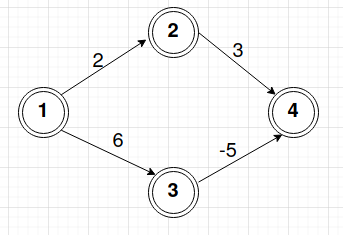
\includegraphics[width=0.55\textwidth]{pic3}
			\caption{Counter example for Dijkstra algorithm}
			\label{fig:mesh1}
		\end{figure}\\
		For the above graph it is easy to see that the shortest path from node 1 to node 4 is $1->3->4$. However, the Dijkstra's algorithm incorrectly finds the path 1 $1->2->4$ by greedily following the minimum weight edges (it will not use node 3 because $6 > 5$).
	
	
	
	\end{enumerate}
\end{document}

